\documentclass{beamer}
\usetheme{metropolis}
\title{InIceMC Meeting - C++ module for RF propagation through Ice and Firn}
\date{\today}
\author{J. C. Hanson (CCAPP, The Ohio State University)}
\institute{CCAPP @ OSU}
\usepackage{outlines}
\usepackage{enumitem}
\usepackage{graphicx}
\usepackage{amsmath}
\setenumerate[1]{label=\Roman*.}
\setenumerate[2]{label=\Alph*.}
\setenumerate[3]{label=\roman*.}
\setenumerate[4]{label=\alph*.}
\newcommand{\sign}{\text{sgn}}
\usepackage{siunitx}

\begin{document} \maketitle
\small

\begin{frame}{Outline}
\begin{outline}[enumerate]
\1 A C++ Module for RF propagation in ice - Why?
\2 Class structure and functions
\2 How Propagator.h works
\1 Physics questions
\2 Measured firn profiles and channeling
\2 Reaching the surface
\2 Air to firn propagation (new)
\2 RFRay.h distance and loss tracking (new)
\1 What's next?
\2 Diffuse reflection (Geoffrey)
\2 Verify with Mathematica (Spoorti)
\2 Channelling with no explicit reflection layer
\end{outline}
\end{frame}

\section{The Code}

\begin{frame}{Class Structure and Functions - see Github, 918particle, Ray Propagation}
\begin{figure}
\begin{center}
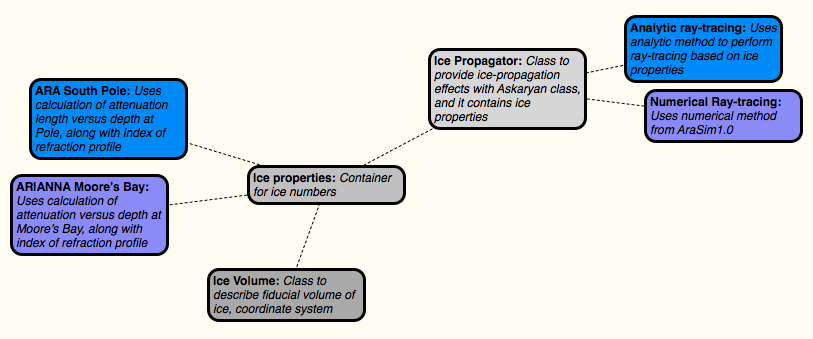
\includegraphics[width=0.9\textwidth]{figures/Propagation.png}
\caption{\label{fig:fig1} The original RF propagation class structure from AraSim2 outline.}
\end{center}
\end{figure}
\end{frame}

\begin{frame}{Class Structure and Functions}
\begin{figure}
\begin{center}
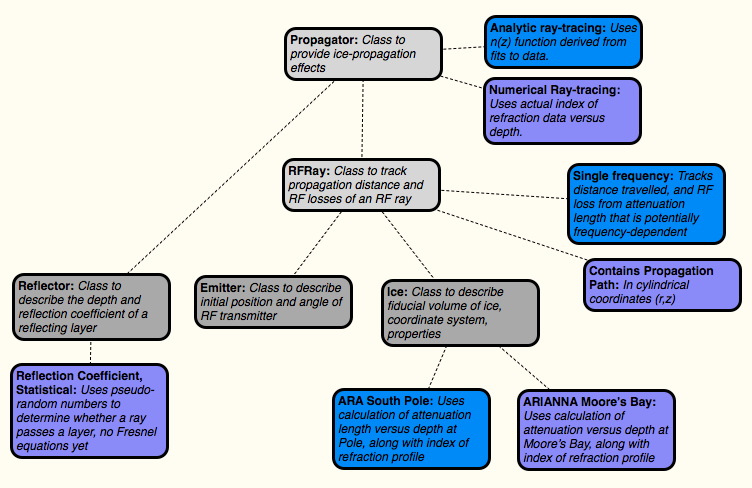
\includegraphics[width=0.8\textwidth]{figures/Propagation2.png}
\caption{\label{fig:fig2} The current RF propagation class structure.}
\end{center}
\end{figure}
\end{frame}

\begin{frame}[fragile]{How Propagator.h Works}
\small
\begin{verbatim}
class Propagator : public Reflector, public RFRay
{
public:
float _globalTime; //nanoseconds
float _timeStep; //nanoseconds
std::pair<float,float> _currentPosition;
bool _isInitialized;
...
void InitializePropagator(float,...,float);
void AddReflector(float,float);
void Propagate(); //Propagate ray through medium
void ReadoutPath(std::string);
};
\end{verbatim}
\end{frame}

\begin{frame}[fragile]{How Propagator.h Works - Check for reflections (issue no. 1)}
\tiny
\begin{verbatim}
void Propagator::Propagate()
{
float c0 = 0.299792458; //speed of light in vacuum, meters per nanosecond
float dz = 1.0e-4; //units: meters
float dndz = 0.0; //units: meters^(-1)
float theTime = 0.0;
this->_path.push_back(_emitterPosition);
bool flag = true;
while(theTime<_globalTime)
{
 float n = GetIndex(_emitterPosition.second);
 theTime+=_timeStep;
 std::pair<float,float> old_pos = _emitterPosition;
 _emitterPosition.first+=cos(_initialAngle)*_timeStep*c0/n;
 _emitterPosition.second+=sin(_initialAngle)*_timeStep*c0/n;
 this->_path.push_back(_emitterPosition);
 CheckForAReflection(_initialAngle,_emitterPosition.second);
...
\end{verbatim}
\end{frame}

\begin{frame}[fragile]{How Propagator.h Works - Evaluate $dn/dz$ (issue no. 2)}
\tiny
\begin{verbatim}
...
 if(std::abs(old_pos.second-_emitterPosition.second)>dz)
 {
  dndz = (GetIndex(_emitterPosition.second)-GetIndex(old_pos.second))
   /(_emitterPosition.second-old_pos.second);
  }
  else
  {
   dndz = (GetIndex(_emitterPosition.second)-GetIndex(_emitterPosition.second-dz))
   /(_emitterPosition.second-dz);
  }
  float dTheta = _timeStep*cos(_initialAngle)*dndz*c0/(n*n);
  std::cout<<dTheta*180.0/3.14159<<" ";
  if(dTheta>=3.14159/2.0 && dTheta<3.14159) dTheta-=3.14159/2.0;
  else if(dTheta>=3.14159) dTheta-=3.14159;
  _initialAngle+=dTheta;
  this->_currentAngle = _initialAngle; //Change this after today, May 19th, 2017.
  }
}
\end{verbatim}
\end{frame}

\section{Physics Questions}

\begin{frame}{Measured Firn Profiles and Channelling}
\begin{figure}
\begin{center}
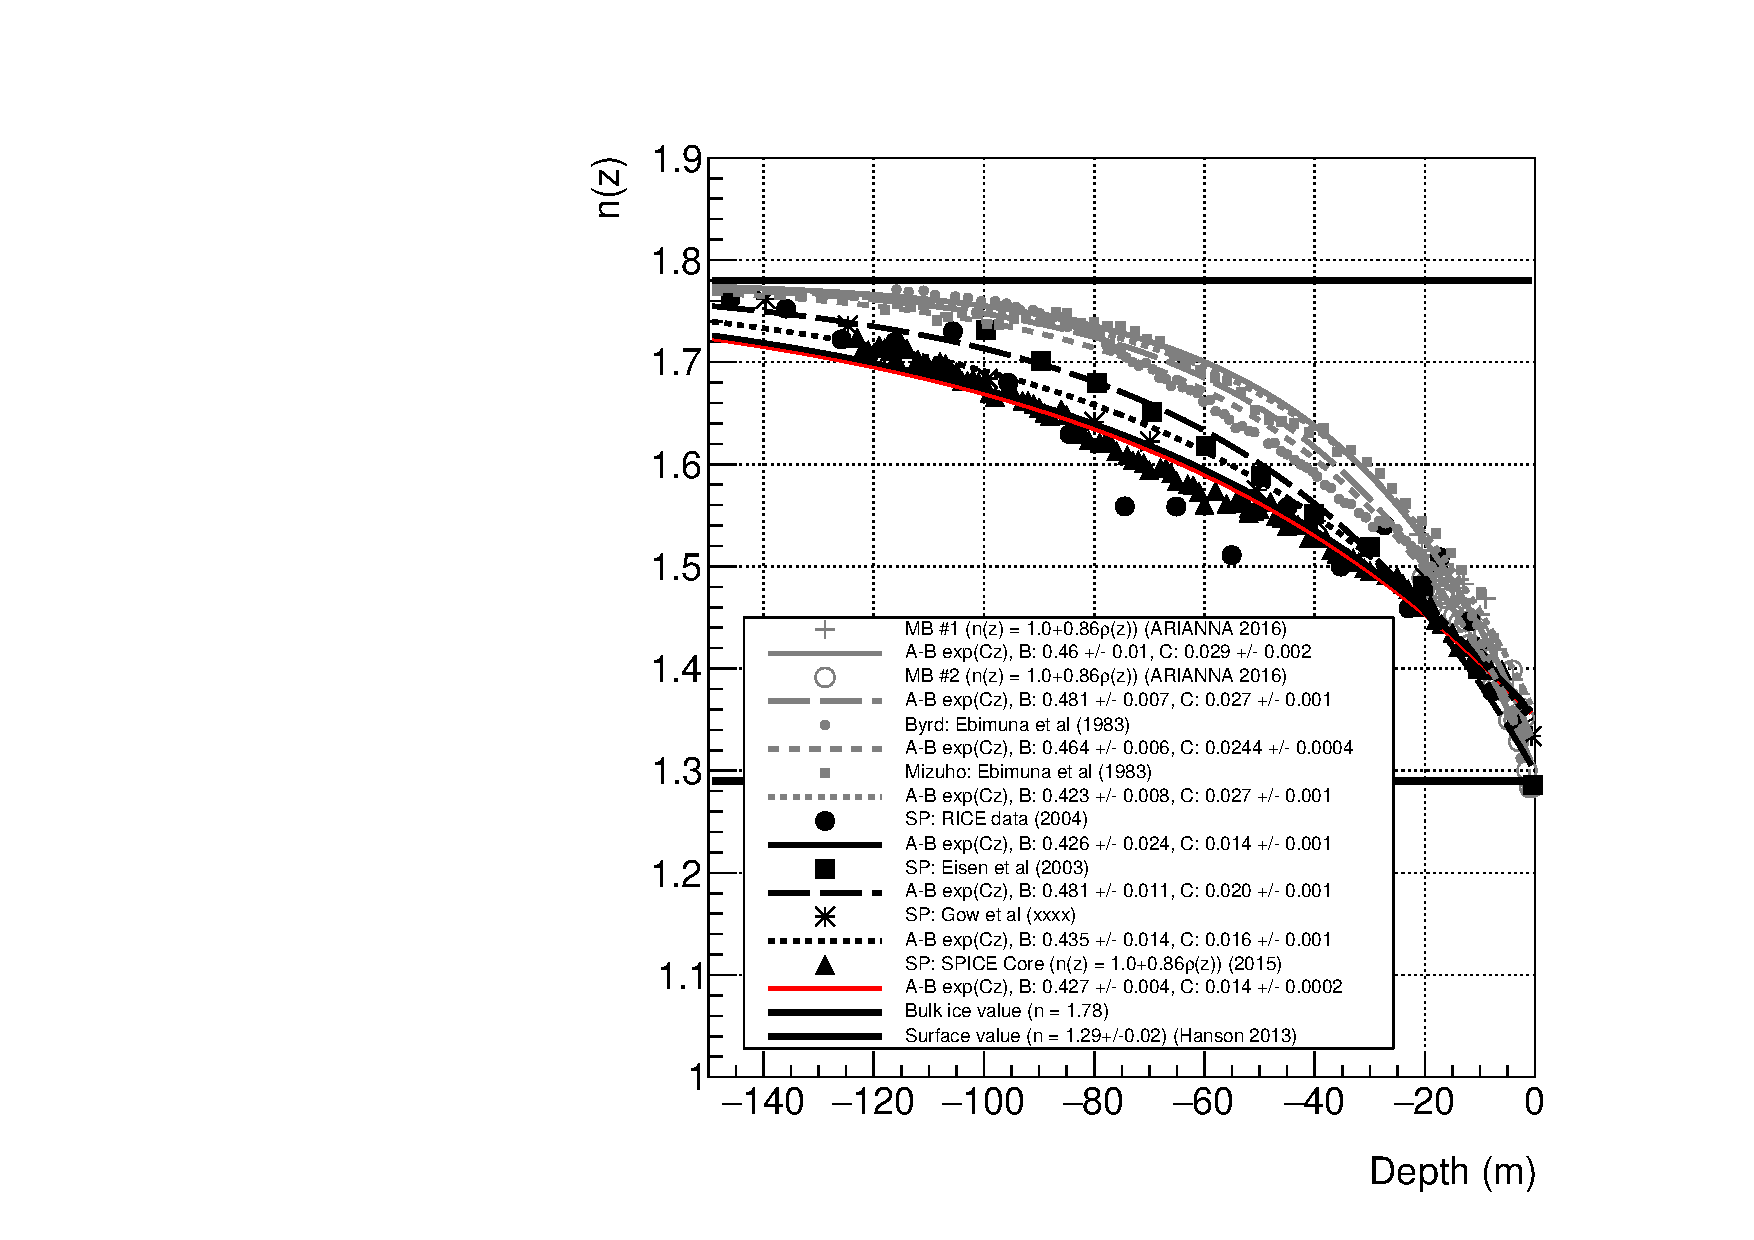
\includegraphics[width=0.6\textwidth,angle=270]{figures/April21_plot1.pdf}
\caption{\label{fig:fig3} Summary of index of refraction data and fits.}
\end{center}
\end{figure}
\end{frame}

\begin{frame}[fragile]{Measured Firn Profiles and Channelling}
\begin{verbatim}
else if(modelName=="Gow")
{
_A = 1.78;
_B = 0.435;
_C = 0.016;
std::ifstream in("/home/jordan/ANewHope/Gow_withOnePlus86_data.csv");
float depth,index;
while(in.good() && ~in.eof())
{
in>>depth;
in>>index;
_indexVsDepth.push_back(std::pair<float,float>(depth,index));
}
in.close();
}
\end{verbatim}
\end{frame}

\begin{frame}{Reaching the Surface with Refraction and Chanelling}
\begin{figure}
\begin{center}
\includegraphics[width=0.5\textwidth,angle=270]{/Users/918particle/Ray_Propagation/code/cpp_propagation/latest_plots/May11/May11_plot2.eps}
\caption{\label{fig:fig4} Index profile is a $n(z)$ function.}
\end{center}
\end{figure}
\end{frame}

\begin{frame}{Reaching the Surface with Refraction and Chanelling}
\begin{figure}
\begin{center}
\includegraphics[width=0.5\textwidth,angle=270]{/Users/918particle/Ray_Propagation/code/cpp_propagation/latest_plots/May11/May11_plot3.eps}
\caption{\label{fig:fig5} Index profile is linear interpolation of data.}
\end{center}
\end{figure}
\end{frame}

\begin{frame}{Reaching the Surface with Refraction and Chanelling}
\begin{figure}
\begin{center}
\includegraphics[width=0.5\textwidth,angle=270]{/Users/918particle/Ray_Propagation/code/cpp_propagation/latest_plots/May18/May18_plot1_testSurfaceTransmission.eps}
\caption{\label{fig:fig6} Varying the angle to test propagation to surface.}
\end{center}
\end{figure}
\end{frame}

\begin{frame}{Reaching the Surface with Refraction and Chanelling}
\begin{figure}
\begin{center}
\includegraphics[width=0.5\textwidth,angle=270]{/Users/918particle/Ray_Propagation/code/cpp_propagation/latest_plots/May18/May18_plot2_testSurfaceTransmission.eps}
\caption{\label{fig:fig7} Varying the angle to test propagation to surface.}
\end{center}
\end{figure}
\end{frame}

\begin{frame}{Reaching the Surface with Refraction and Chanelling}
\begin{figure}
\begin{center}
\includegraphics[width=0.5\textwidth,angle=270]{/Users/918particle/Ray_Propagation/code/cpp_propagation/latest_plots/May18/May18_plot3_testSurfaceTransmission.eps}
\caption{\label{fig:fig8} Varying the angle to test propagation to surface.}
\end{center}
\end{figure}
\end{frame}

\begin{frame}{Reaching the Surface with Refraction and Chanelling}
\begin{figure}
\begin{center}
\includegraphics[width=0.5\textwidth,angle=270]{/Users/918particle/Ray_Propagation/code/cpp_propagation/latest_plots/May18/May18_plot4_testSurfaceTransmission.eps}
\caption{\label{fig:fig9} Varying the angle to test propagation to surface.}
\end{center}
\end{figure}
\end{frame}

\begin{frame}{Reaching the Surface with Refraction and Chanelling}
\begin{figure}
\begin{center}
\includegraphics[width=0.5\textwidth,angle=270]{/Users/918particle/Ray_Propagation/code/cpp_propagation/latest_plots/May18/May18_plot5_testSurfaceTransmission.eps}
\caption{\label{fig:fig10} Varying the angle to test propagation to surface.}
\end{center}
\end{figure}
\end{frame}

\begin{frame}{Reaching the Surface with Refraction and Chanelling}
\begin{figure}
\begin{center}
\includegraphics[width=0.5\textwidth,angle=270]{/Users/918particle/Ray_Propagation/code/cpp_propagation/latest_plots/May18/May18_plot6_testSurfaceTransmission.eps}
\caption{\label{fig:fig11} Varying the angle to test propagation to surface.}
\end{center}
\end{figure}
\end{frame}

\begin{frame}{Signals from Air to Firn}
\begin{figure}
\begin{center}
\includegraphics[width=0.5\textwidth,angle=270]{/Users/918particle/Ray_Propagation/code/cpp_propagation/latest_plots/May18/May18_plot1_testAirTransmission.eps}
\caption{\label{fig:fig12} Varying the angle to test propagation to from air to firn.}
\end{center}
\end{figure}
\end{frame}

\begin{frame}{Signals from Air to Firn}
\begin{figure}
\begin{center}
\includegraphics[width=0.5\textwidth,angle=270]{/Users/918particle/Ray_Propagation/code/cpp_propagation/latest_plots/May18/May18_plot2_testAirTransmission.eps}
\caption{\label{fig:fig13} Varying the angle to test propagation to from air to firn.}
\end{center}
\end{figure}
\end{frame}

\begin{frame}{Signals from Air to Firn}
\begin{figure}
\begin{center}
\includegraphics[width=0.5\textwidth,angle=270]{/Users/918particle/Ray_Propagation/code/cpp_propagation/latest_plots/May18/May18_plot3_testAirTransmission.eps}
\caption{\label{fig:fig14} Varying the angle to test propagation to from air to firn.}
\end{center}
\end{figure}
\end{frame}

\begin{frame}{Signals from Air to Firn}
\begin{figure}
\begin{center}
\includegraphics[width=0.5\textwidth,angle=270]{/Users/918particle/Ray_Propagation/code/cpp_propagation/latest_plots/May18/May18_plot4_testAirTransmission.eps}
\caption{\label{fig:fig15} Varying the angle to test propagation to from air to firn.}
\end{center}
\end{figure}
\end{frame}

\begin{frame}{Signals from Air to Firn}
\begin{figure}
\begin{center}
\includegraphics[width=0.5\textwidth,angle=270]{/Users/918particle/Ray_Propagation/code/cpp_propagation/latest_plots/May18/May18_plot5_testAirTransmission.eps}
\caption{\label{fig:fig16} Varying the angle to test propagation to from air to firn.}
\end{center}
\end{figure}
\end{frame}

\begin{frame}{Signals from Air to Firn}
\begin{figure}
\begin{center}
\includegraphics[width=0.5\textwidth,angle=270]{/Users/918particle/Ray_Propagation/code/cpp_propagation/latest_plots/May18/May18_plot6_testAirTransmission.eps}
\caption{\label{fig:fig17} Varying the angle to test propagation to from air to firn.}
\end{center}
\end{figure}
\end{frame}

\begin{frame}[fragile]{How Propagator.h Works}
\small 
\begin{verbatim}
class RFRay : public Emitter, public Ice
{
public:
RFRay() : _distanceTravelled(0.0), _rfLoss(0.0), _freq(0.0){};
void SetFreq(float);
void Update(std::pair<float,float>,float);
std::pair<float,float> _currentPosition; //Current position in (x,z)
float _currentAngle; //Current angle with respect to horizontal
std::pair<float,float> _priorPosition; //Current position in (x,z)
float _distanceTravelled; //Keeps track of the propagation distance
float _rfLoss; //Amount of attenuation (apart from distance) accumulated
float _freq; //Frequency of the ray
std::vector<std::pair<float,float> > _path;
};
\end{verbatim}
\end{frame}

\begin{frame}{Outline}
\begin{outline}[enumerate]
\1 A C++ Module for RF propagation in ice - Why?
\2 Class structure and functions
\2 How Propagator.h works
\1 Physics questions
\2 Measured firn profiles and channeling
\2 Reaching the surface
\2 Air to firn propagation (new)
\2 RFRay.h distance and loss tracking (new)
\1 \textbf{What's next?}
\2 \textbf{Diffuse reflection (Geoffrey)}
\2 \textbf{Verify with Mathematica (Spoorti)}
\2 \textbf{Channelling with no explicit reflection layer}
\end{outline}
\end{frame}

\end{document}